\subsubsection{} Подтверждение номера телефона
\label{sec:usage:auth:sms}

После успешной проверки номера телефона (выполняется на~сервере), на~телефон отправляется смс сообщение с~кодом подтверждения номера, а~приложение переходит на~экран подтверждения номера телефона \ref{sec:usage:auth:sms:confirm}. Пользователь должен ввести код из~смс в~поле <<Код подтверждения>> и~нажать кнопку <<Войти>>.

\begin{figure}[h]
  \centering
    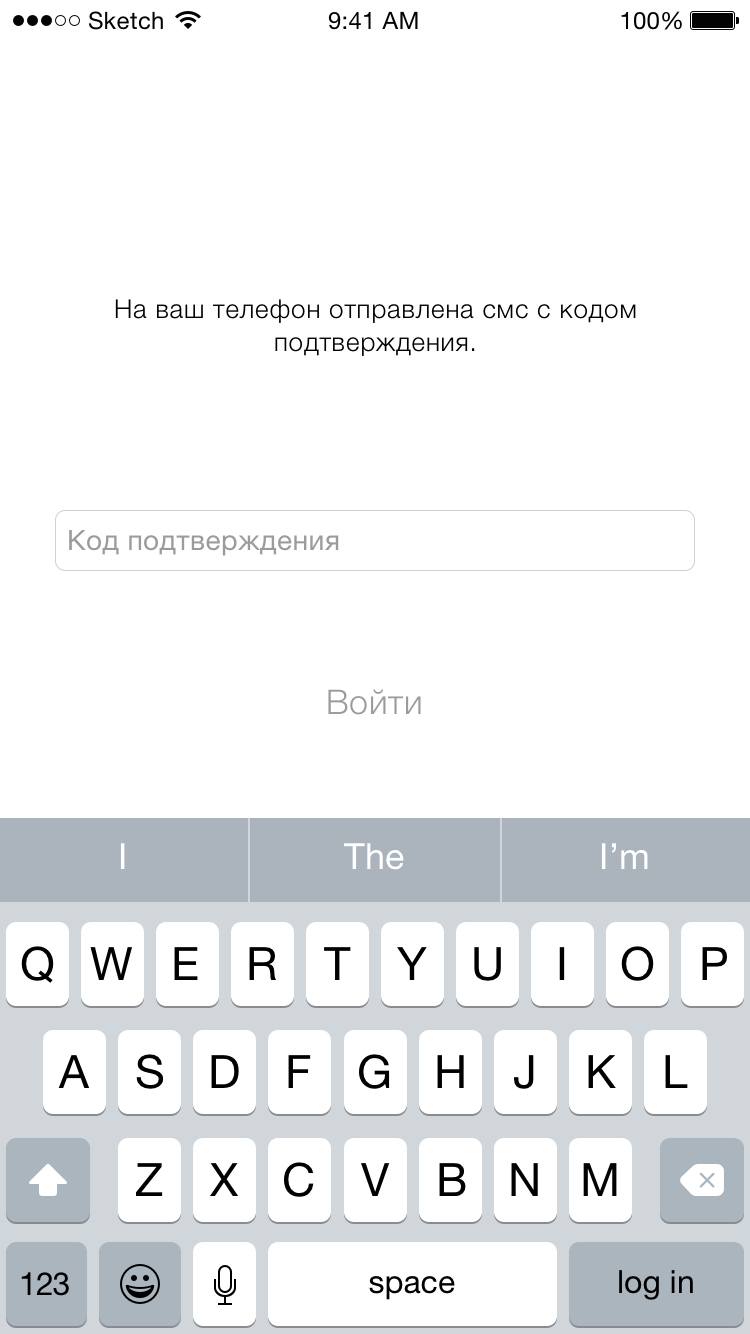
\includegraphics[height=0.25\textheight]{inc/img/ui/sms_not_entered.png}
  \caption{Экран подтверждения номера телефона}
  \label{sec:usage:auth:sms:confirm}
\end{figure}